\documentclass[aspectratio=169,11pt]{beamer}

% Compile with pdfLaTeX. Sources reviewed on 2026-11-09.
% Sheet: https://docs.google.com/spreadsheets/d/1aQGHk3CCcypYjSrMD-Z9yHB_KMrWZ5OGlXp1mt-CLV8/edit
% Code snapshots: hardware 8e0a5a3, mobile 23ecf5a, firmware core 6f2c13e.
% Tracker status, code implementation and physical acceptance are reported separately.
\usepackage[utf8]{inputenc}
\usepackage[T5,T1]{fontenc}
\usepackage[english]{babel}
\usepackage{lmodern}
\usepackage{graphicx}
\usepackage{booktabs}
\usepackage{tabularx}
\usepackage{tikz}
\usetikzlibrary{arrows.meta}
% Prefer updated project assets. Root uploads also work on Overleaf.
\graphicspath{{report/}{./}}

\definecolor{DeepBlue}{HTML}{003B70}
\definecolor{AccentRed}{HTML}{C8102E}
\definecolor{BodyInk}{HTML}{202B36}
\definecolor{SoftBlue}{HTML}{EAF1F7}
\setbeamercolor{normal text}{fg=BodyInk,bg=white}
\setbeamercolor{structure}{fg=DeepBlue}
\setbeamercolor{frametitle}{fg=white}
\setbeamercolor{title}{fg=DeepBlue}
\setbeamercolor{block title}{fg=white,bg=DeepBlue}
\setbeamercolor{block body}{fg=BodyInk,bg=SoftBlue}
\setbeamerfont{frametitle}{series=\bfseries,size=\Large}
\setbeamertemplate{navigation symbols}{}
\setbeamertemplate{itemize item}{\color{AccentRed}\textbullet}
\setbeamertemplate{itemize subitem}{\color{AccentRed}--}
% Reserve the template's top band and its logo/footer area.
\setbeamertemplate{headline}{\vspace*{1.25cm}}
\setbeamertemplate{frametitle}{%
  \begin{tikzpicture}[remember picture,overlay]
    \node[anchor=west,inner sep=0pt,text=white,text width=14.2cm,
      font=\bfseries\fontsize{17}{20}\selectfont]
      at ([xshift=0.85cm,yshift=-0.39cm]current page.north west)
      {\insertframetitle};
  \end{tikzpicture}%
}
\setbeamertemplate{footline}{%
  \vbox{%
    \vspace*{0.72cm}%
    \hbox to \paperwidth{\hfill
      {\color{DeepBlue}\fontsize{8}{10}\selectfont\insertframenumber/\inserttotalframenumber}%
      \hspace*{0.65cm}}%
    \vspace*{0.12cm}%
  }%
}
\setbeamersize{text margin left=9mm,text margin right=9mm}
\setlength{\parskip}{0.35em}
\renewcommand{\arraystretch}{1.18}

\newcommand{\GroupName}{Project Team}
\newcommand{\VNname}[1]{{\fontencoding{T5}\selectfont #1}}
\newcommand{\SheetLink}{https://docs.google.com/spreadsheets/d/1aQGHk3CCcypYjSrMD-Z9yHB_KMrWZ5OGlXp1mt-CLV8/edit}
\newcommand{\RepoLink}{https://github.com/itstheblank/esp32_smart_home}

% Upload background.png next to main.tex to apply the background to every slide.
\IfFileExists{background.png}{%
  \usebackgroundtemplate{
\includegraphics[width=\paperwidth,height=\paperheight]{background.png}}%
}{%
  \usebackgroundtemplate{%
    \begin{tikzpicture}[remember picture,overlay]
      \fill[DeepBlue] (current page.north west)
        rectangle ([yshift=-0.78cm]current page.north east);
      \draw[AccentRed,line width=1.2pt]
        ([yshift=-0.97cm]current page.north west) --
        ([yshift=-0.97cm]current page.north east);
    \end{tikzpicture}%
  }%
}

\title{ESP32 SMART HOME}
\subtitle{Checkpoint 1 --- System Design and Demonstration}
\author{\VNname{Trần Sỹ Nguyên} \and \VNname{Lăng Hồng Nguyệt Anh} \and \VNname{Lương Ngọc Vũ Long} \and \VNname{Hà Đức Dương} \and \VNname{Nguyễn Vũ Anh Khoa}}
\date{9 November 2026}

\begin{document}

\begin{frame}{CHECKPOINT 1}
  \begingroup
  \setlength{\parskip}{0pt}
  \vfill
  {\fontsize{28}{32}\selectfont\color{DeepBlue}\bfseries ESP32 SMART HOME}\par
  \vspace{0.18cm}
  {\large System Design and Demonstration}\par
  \vspace{0.45cm}
  {\normalsize\bfseries \GroupName}\par
  \vspace{0.15cm}
  {\small\renewcommand{\arraystretch}{1.3}
    \begin{tabular}{@{}p{5.1cm}r@{}}
      \VNname{Trần Sỹ Nguyên} & 20235985 \\
      \VNname{Lăng Hồng Nguyệt Anh} & 20235885 \\
      \VNname{Lương Ngọc Vũ Long} & 20235967 \\
      \VNname{Hà Đức Dương} & 20235923 \\
      \VNname{Nguyễn Vũ Anh Khoa} & 20235957 \\
    \end{tabular}\par
  }
  \vspace{0.3cm}
  \vfill
  \endgroup
\end{frame}

\begin{frame}{Presentation Outline}
  \vfill
  {\Large\bfseries\color{AccentRed} 01}\quad {\large\bfseries Introduction}\par
  \vspace{0.45cm}
  {\Large\bfseries\color{AccentRed} 02}\quad {\large\bfseries Requirements}\par
  \vspace{0.45cm}
  {\Large\bfseries\color{AccentRed} 03}\quad {\large\bfseries System Design}\par
  \vspace{0.45cm}
  {\Large\bfseries\color{AccentRed} 04}\quad {\large\bfseries Budget}\par
  \vspace{0.45cm}
  {\Large\bfseries\color{AccentRed} 05}\quad {\large\bfseries Progress and Demo}\par
  \vspace{0.45cm}
  {\Large\bfseries\color{AccentRed} 06}\quad {\large\bfseries Team and Status}\par
  \vfill
\end{frame}

\begin{frame}{1. Problem and Users}
  \small
  \begin{block}{The problem}
    In most homes, turning on a light still means walking to the switch.
    Even with a smart app, you still have to press the button yourself ---
    there is no way to tell the system when the light should turn on, so it
    can never act automatically.
  \end{block}
  \vspace{0.1cm}
  \small
  \begin{columns}[T,onlytextwidth]
    \begin{column}{0.47\textwidth}
      {\large\bfseries\color{DeepBlue} Intended users}\par
      Homeowners and renters who want everyday devices controllable from a phone, with no technical knowledge required.
    \end{column}
    \begin{column}{0.48\textwidth}
      {\large\bfseries\color{DeepBlue} Why it matters}\par
      \begin{itemize}
        \item Control devices without going to each switch.
        \item See device state live, with history for monitoring.
        \item Automate device control through customizable rules.
      \end{itemize}
    \end{column}
  \end{columns}
\end{frame}

\begin{frame}{1. Checkpoint 1 Scope}
  \footnotesize
  \setlength{\parskip}{0.2em}
  \begin{columns}[T,onlytextwidth]
    \begin{column}{0.48\textwidth}
      {\large\bfseries\color{DeepBlue} In scope now}\par
      \begin{itemize}
        \item Light ON/OFF and door open/close over MQTT
          (\texttt{smarthome/cmd}) from the web dashboard.
        \item PIR motion turns the light on, auto-off after inactivity.
        \item RFID allowlist opens the door; unknown cards are rejected and
          logged.
        \item Live web dashboard: SSE stream of the last 300 events, device
          state at a glance.
        \item Rules engine: trigger/condition/action rules, persisted in
          \texttt{rules.json} across restarts.
      \end{itemize}
    \end{column}
    \begin{column}{0.48\textwidth}
      {\large\bfseries\color{DeepBlue} Deliberately deferred}\par
      \begin{itemize}
        \item Mobile app on the unified contract --- alignment with the
          refactored topics is in progress.
        \item Voice control (planned after core acceptance).
        \item Database-backed event history; logs stay in a RAM buffer
          (only rules persist).
        \item Cloud/remote access; the demo runs on a shared LAN.
        \item Energy-saving measurement.
      \end{itemize}
    \end{column}
  \end{columns}
\end{frame}

\begin{frame}{2. Functional Requirements}
  \small
  \begin{tabularx}{\textwidth}{@{}lX@{}}
    \toprule
    \textbf{ID} & \textbf{What the system must do} \\
    \midrule
    FR1 & Turn the light ON and OFF from the dashboard, with the real state confirmed back. \\
    FR2 & Open and close the model door remotely. \\
    FR3 & Turn the light on when motion is detected, and off again by itself after a configurable quiet period. \\
    FR4 & Open the door only for RFID cards on the allowlist; reject and log everyone else. \\
    FR5 & Show the live state of the light, door, motion sensor and connection on one screen. \\
    FR6 & Keep a running list of recent sensor readings, access attempts and device events. \\
    \bottomrule
  \end{tabularx}
\end{frame}

\begin{frame}{2. Non-functional Targets}
  \footnotesize
  \renewcommand{\arraystretch}{1.05}
  \begin{tabularx}{\textwidth}{@{}lp{2.6cm}X@{}}
    \toprule
    \textbf{ID} & \textbf{Quality} & \textbf{What counts as passing} \\
    \midrule
    NFR1 & Stability & Runs 30 minutes with no reset and no dropped connection. \\
    NFR2 & Mechanism & Door completes 20 open/close cycles without jamming. \\
    NFR3 & Recovery & After a broker or Wi-Fi outage, the ESP32 reconnects and resumes its state. \\
    NFR4 & Robustness & Malformed commands are rejected and logged; firmware keeps running. \\
    NFR5 & Repeatability & Every must-have scenario passes twice in a row. \\
    \bottomrule
  \end{tabularx}
  \vspace{0.35cm}
  {\small Each target is checked with a short, repeatable test on the physical model --- the results are shown at the demo.}
\end{frame}

\begin{frame}{3. Architecture}
  \centering
  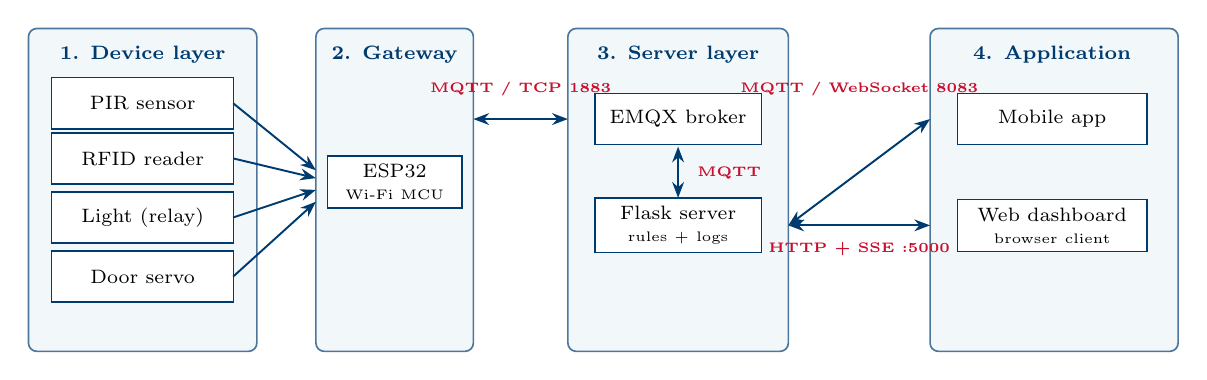
\begin{tikzpicture}[
      font=\scriptsize,
      layerbox/.style={rounded corners=3pt, draw=DeepBlue!70, line width=0.6pt, fill=SoftBlue!60},
      comp/.style={rectangle, draw=DeepBlue, line width=0.5pt, fill=white, align=center,
        inner sep=3pt, minimum height=6.5mm, text width=2.1cm},
      conn/.style={{Stealth[length=2mm]}-{Stealth[length=2mm]}, line width=0.7pt, DeepBlue},
      one/.style={{Stealth[length=2mm]}-, line width=0.7pt, DeepBlue},
      hoplab/.style={font=\tiny\bfseries, text=AccentRed, align=center}
    ]
    % ---------- 1. Device layer
    \draw[layerbox] (0.05,-2.05) rectangle (2.95,2.05);
    \node[font=\scriptsize\bfseries, text=DeepBlue] at (1.5,1.72) {1. Device layer};
    \node[comp] (pir)   at (1.5, 1.10) {PIR sensor};
    \node[comp] (rfid)  at (1.5, 0.40) {RFID reader};
    \node[comp] (light) at (1.5,-0.35) {Light (relay)};
    \node[comp] (servo) at (1.5,-1.10) {Door servo};

    % ---------- 2. Gateway layer
    \draw[layerbox] (3.7,-2.05) rectangle (5.7,2.05);
    \node[font=\scriptsize\bfseries, text=DeepBlue] at (4.7,1.72) {2. Gateway};
    \node[comp, text width=1.5cm] (esp) at (4.7,0.1) {ESP32{\tiny\\ Wi-Fi MCU}};

    % ---------- 3. Server layer
    \draw[layerbox] (6.9,-2.05) rectangle (9.7,2.05);
    \node[font=\scriptsize\bfseries, text=DeepBlue] at (8.3,1.72) {3. Server layer};
    \node[comp, text width=1.9cm] (emqx)  at (8.3, 0.90) {EMQX broker};
    \node[comp, text width=1.9cm] (flask) at (8.3,-0.45) {Flask server{\tiny\\ rules + logs}};

    % ---------- 4. Application layer
    \draw[layerbox] (11.5,-2.05) rectangle (14.65,2.05);
    \node[font=\scriptsize\bfseries, text=DeepBlue] at (13.05,1.72) {4. Application};
    \node[comp, text width=2.2cm] (mobile) at (13.05, 0.90) {Mobile app};
    \node[comp, text width=2.2cm] (web)    at (13.05,-0.45) {Web dashboard{\tiny\\ browser client}};

    % ---------- device <-> gateway wiring
    \draw[one] (3.7,0.25) -- (2.65, 1.10);
    \draw[one] (3.7,0.15) -- (2.65, 0.40);
    \draw[one] (3.7,0.00) -- (2.65,-0.35);
    \draw[one] (3.7,-0.15) -- (2.65,-1.10);

    % ---------- gateway <-> server
    \draw[conn] (5.7,0.90) -- (6.9,0.90);
    \node[hoplab] at (6.3,1.28) {MQTT / TCP 1883};

    % ---------- inside server
    \draw[conn] (8.3,0.55) -- (8.3,-0.10);
    \node[hoplab, anchor=west] at (8.42,0.22) {MQTT};

    % ---------- server <-> application
    \draw[conn] (9.7,-0.45) -- (11.5,0.90);
    \node[hoplab] at (10.6,1.28) {MQTT / WebSocket 8083};
    \draw[conn] (9.7,-0.45) -- (11.5,-0.45);
    \node[hoplab] at (10.6,-0.75) {HTTP + SSE :5000};
  \end{tikzpicture}

  \vspace{0.15cm}
\end{frame}

\begin{frame}{3. MQTT Contract per Hop}
  \small
  \begin{tabularx}{\textwidth}{@{}p{2.8cm}XX@{}}
    \toprule
    & \textbf{Unified contract (firmware + server)} & \textbf{Mobile branch (not yet updated)} \\
    \midrule
    Command topic & \texttt{smarthome/cmd}, one JSON command for every device & \texttt{smarthome/cmd/light}\newline\texttt{smarthome/cmd/door} as plain text \\
    Feedback topics & \texttt{smarthome/logs}, one stream for states and events & \texttt{smarthome/state/+}\newline\texttt{smarthome/event/access} \\
    Payload & JSON for both commands and logs & Text commands, mixed JSON events \\
    Transport & TCP 1883 for devices and the server & WebSocket 8083 for the app \\
    \bottomrule
  \end{tabularx}
  \vspace{0.35cm}
  \textcolor{AccentRed}{\bfseries Integration priority}\quad Both transports are fine --- only topics and payloads have to match. Updating the mobile branch is the top integration task.
\end{frame}

\begin{frame}{3. Technology Choices and Rationale}
  \small
  \begingroup
  \renewcommand{\arraystretch}{1.25}
  \hyphenpenalty=10000
  \exhyphenpenalty=10000
  \begin{tabularx}{\textwidth}{@{}>{\raggedright\arraybackslash}p{3.4cm}>{\raggedright\arraybackslash}X@{}}
    \toprule
    \textbf{Technology} & \textbf{Why we picked it} \\
    \midrule
    ESP32 / PlatformIO & One cheap chip drives every sensor and actuator and has Wi-Fi built in. \\
    MQTT / EMQX & Pub/sub decouples devices, server and app; EMQX serves TCP and WebSocket from one broker. \\
    Flask + Paho (Python) & A small server is enough for the rules engine, live log stream (SSE) and dashboard. \\
    React Native / Expo & One codebase for both phones; MQTT over WebSocket connects straight to the broker. \\
    Docker Compose & Broker and server start with a single command on any laptop. \\
    Storage & Rules persist in \texttt{rules.json}; recent events stay in a RAM buffer of 300. \\
    \bottomrule
  \end{tabularx}
  \endgroup
\end{frame}

% Availability and listed amounts follow the hardware list supplied by the team.
% Already available components have no additional purchase cost in this budget.
\begin{frame}{4. Bill of Materials}
  \fontsize{9}{10.5}\selectfont
  \setlength{\parskip}{0.15em}
  \renewcommand{\arraystretch}{1.0}
  \begin{tabularx}{\textwidth}{@{}>{\raggedright\arraybackslash}Xr@{}}
    \toprule
    \textbf{Component / set} & \textbf{Availability / budget (VND)} \\
    \midrule
    ESP32 WT-01 (Ethernet and Wi-Fi) & Available \\
    USB--TTL CH340 adapter & Available \\
    MB-102 breadboard & Available \\
    SG90 servo & 46,116 \\
    RC522 RFID module & Available \\
    5V relay & Available \\
    HC-SR501 PIR sensor & 34,560 \\
    LM2596 buck module & 45,144 \\
    Jumper wires (three types) & Available \\
    12V 2A adapter & 46,116 \\
    DC power jack & 11,124 \\
    \midrule
    \textbf{Budget for remaining items} & \textbf{183,060} \\
    \bottomrule
  \end{tabularx}
  \par\vspace{0.05cm}
  {\footnotesize\raggedright Most parts were already owned; the remaining spend is 183,060 VND (about 7 USD) --- a fraction of a commercial smart-home kit.\par}
\end{frame}

\begin{frame}{5. End-to-end Data Flow}
  \centering
  \vfill
  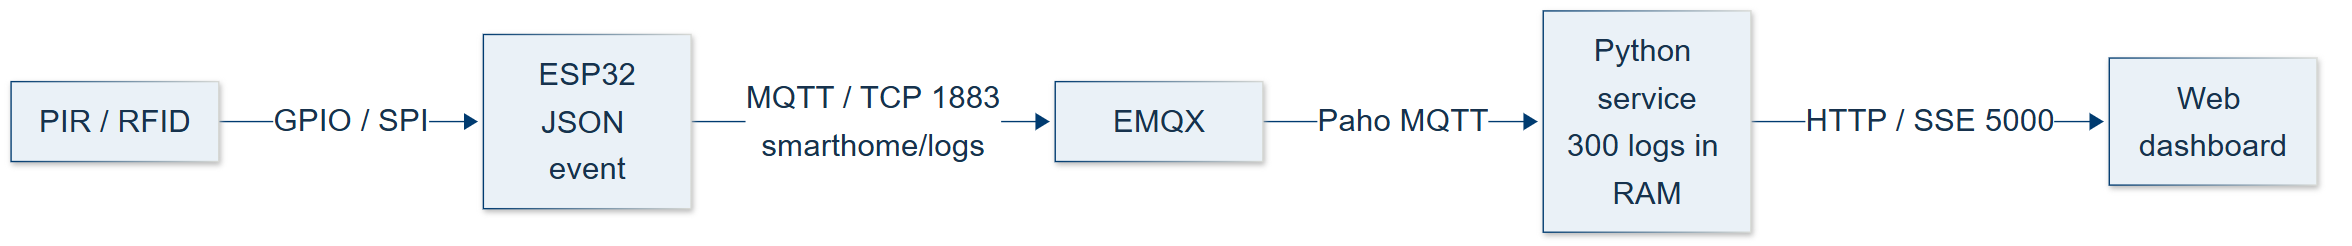
\includegraphics[width=\textwidth,height=0.47\textheight,keepaspectratio]{mqtt-flow.png}
  \vfill
  \begin{minipage}{\textwidth}
    \small
    PIR and RFID events travel from the ESP32 through the broker into the
    server's log store and appear on the dashboard in real time; commands
    take the same path in reverse. The rules engine evaluates every message
    on the way. Next step: record a live sensor-to-screen demo on the
    physical model.
  \end{minipage}
\end{frame}

\begin{frame}{5. Light Command and State Feedback}
  \centering
  \vfill
  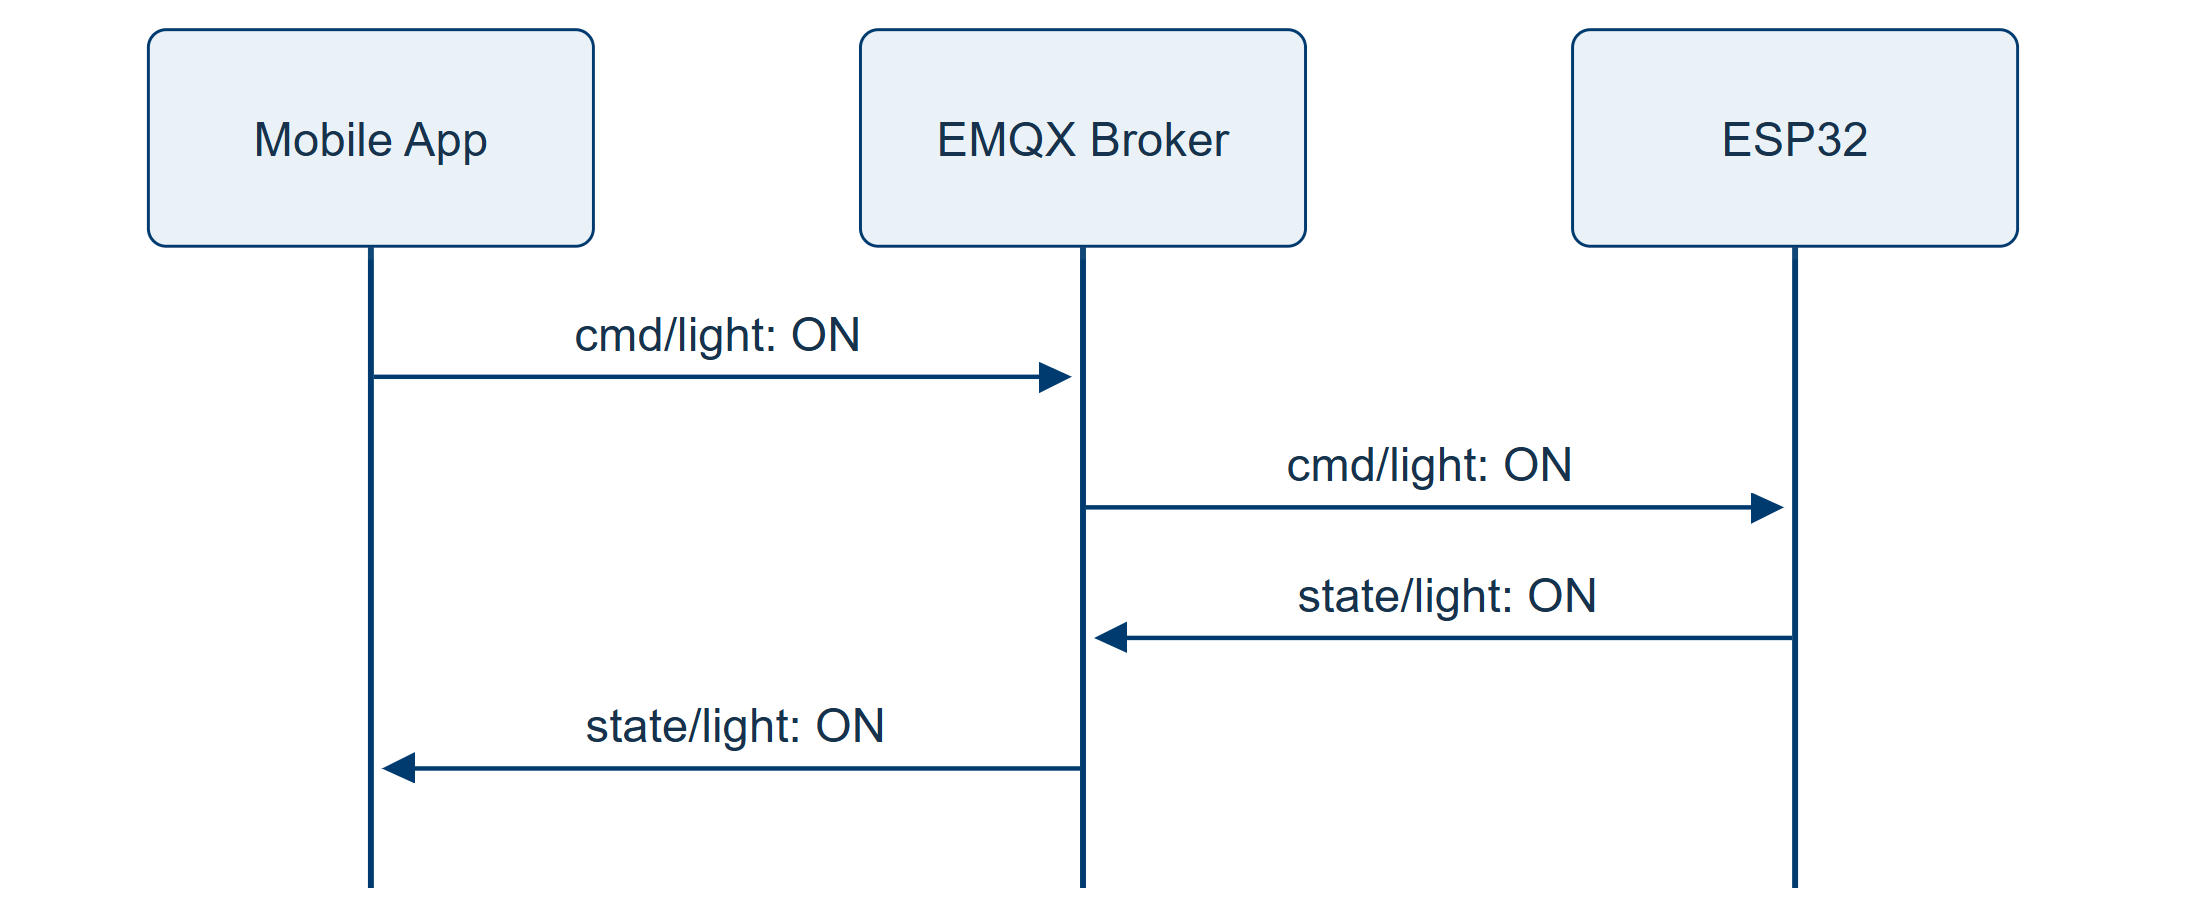
\includegraphics[width=0.93\textwidth,height=0.62\textheight,keepaspectratio]{mqtt-command-flow.png}
  \vfill
  {\small After the refactor there is one command topic in and one log stream back, so the dashboard always shows what the firmware actually did.}
\end{frame}

% Demo assets to be added before the presentation.
\begin{frame}{5. Hardware Demo}
  \centering
  \vfill
  {\Large\color{DeepBlue}\bfseries Hardware Demo}\par
  \vspace{0.4cm}
  {\normalsize Live on the model: PIR-triggered light, RFID door opening and servo actuation, with the dashboard reacting in real time.}
  \vfill
\end{frame}

% Demo assets to be added before the presentation.
\begin{frame}{5. App Demo}
  \centering
  \vfill
  {\Large\color{DeepBlue}\bfseries App Demo}\par
  \vspace{0.4cm}
  {\normalsize Live on screen: sending a command, seeing the state change, scrolling the event log and editing a rule.}
  \vfill
\end{frame}

\begin{frame}{6. Team and Repository}
  \footnotesize
  \setlength{\parskip}{0.2em}
  \begin{tabularx}{\textwidth}{@{}l >{\raggedright\arraybackslash}p{3.9cm} l >{\raggedright\arraybackslash}X@{}}
    \toprule
    \textbf{Member} & \textbf{Name} & \textbf{Student ID} & \textbf{Primary ownership} \\
    \midrule
    M1 & \VNname{Trần Sỹ Nguyên} & 20235985 & Wi-Fi/MQTT core and firmware interfaces \\
    M2 & \VNname{Lăng Hồng Nguyệt Anh} & 20235885 & PIR, RFID authorization and automation \\
    M3 & \VNname{Lương Ngọc Vũ Long} & 20235967 & Power, wiring, actuators and physical model \\
    M4 & \VNname{Hà Đức Dương} & 20235923 & Mobile dashboard, MQTT control and event UI \\
    M5 & \VNname{Nguyễn Vũ Anh Khoa} & 20235957 & Broker, integration, QA and report coordination \\
    \bottomrule
  \end{tabularx}
  \vspace{0.35cm}
  \href{\RepoLink}{\textbf{github.com/itstheblank/esp32\_smart\_home}}\par
\end{frame}

\begin{frame}{6. Top Problems Right Now}
  \small
  \begin{enumerate}
    \item \textbf{Mobile contract drift.} The app branch still publishes the
      old text commands and listens to deprecated topics; it must be migrated
      to \texttt{smarthome/cmd} / \texttt{smarthome/logs} and retested
      end-to-end.
    \item \textbf{No recorded proof of the full loop yet.} The path works in
      code, but we still need a live sensor-to-screen recording on the
      physical model for the demo.
    \item \textbf{Event history is volatile.} Logs live in a RAM buffer of
      300 entries; we have to decide whether checkpoint 2 needs
      database-backed storage.
  \end{enumerate}
\end{frame}

\begin{frame}[plain]
  \centering
  \vfill
  {\Huge\bfseries\color{DeepBlue} Thank You!}\par
  \vspace{0.4cm}
  {\large Questions and Discussion}
  \vfill
\end{frame}

\end{document}
